\subsection{OR問題を学習させた際の誤差収束度合いについて}
\subsubsection{実験結果}
NNでは重みを更新する毎に誤差が減るように学習を行うが、その学習の様子は初期の重みを設定している乱数シード値を1000から100刻みに,10000万まで変更し,実行した.
シード値を変えた際の学習収束回数を表\ref{table:level1}に示す。
シード値を10回変更して学習させた際の重みを更新する様子を図
\ref{fig:level1-1}に、
その平均をプロットした平均推移値を図\ref{fig:level1-2}に示す。


\begin{table}[htb]
 \begin{center}
  \caption{OR問題の学習に要した回数}
  \label{table:level1}
  \begin{tabular}[htb]{r|l} \hline
   シード値 & 収束した回数 \\ \hline \hline
   100 & 96 \\ \hline
   200 & 90 \\ \hline
   300 & 111 \\ \hline
   400 & 109 \\ \hline
   500 & 93 \\ \hline
   600 & 99 \\ \hline
   700 & 100 \\ \hline
   800 & 114 \\ \hline
   900 & 113 \\ \hline
   1000 & 94 \\ \hline \hline
   10試行の平均値 & 101.9 \\ \hline
  \end{tabular}
 \end{center}
\end{table}




\begin{figure}[h]
 \begin{center}
  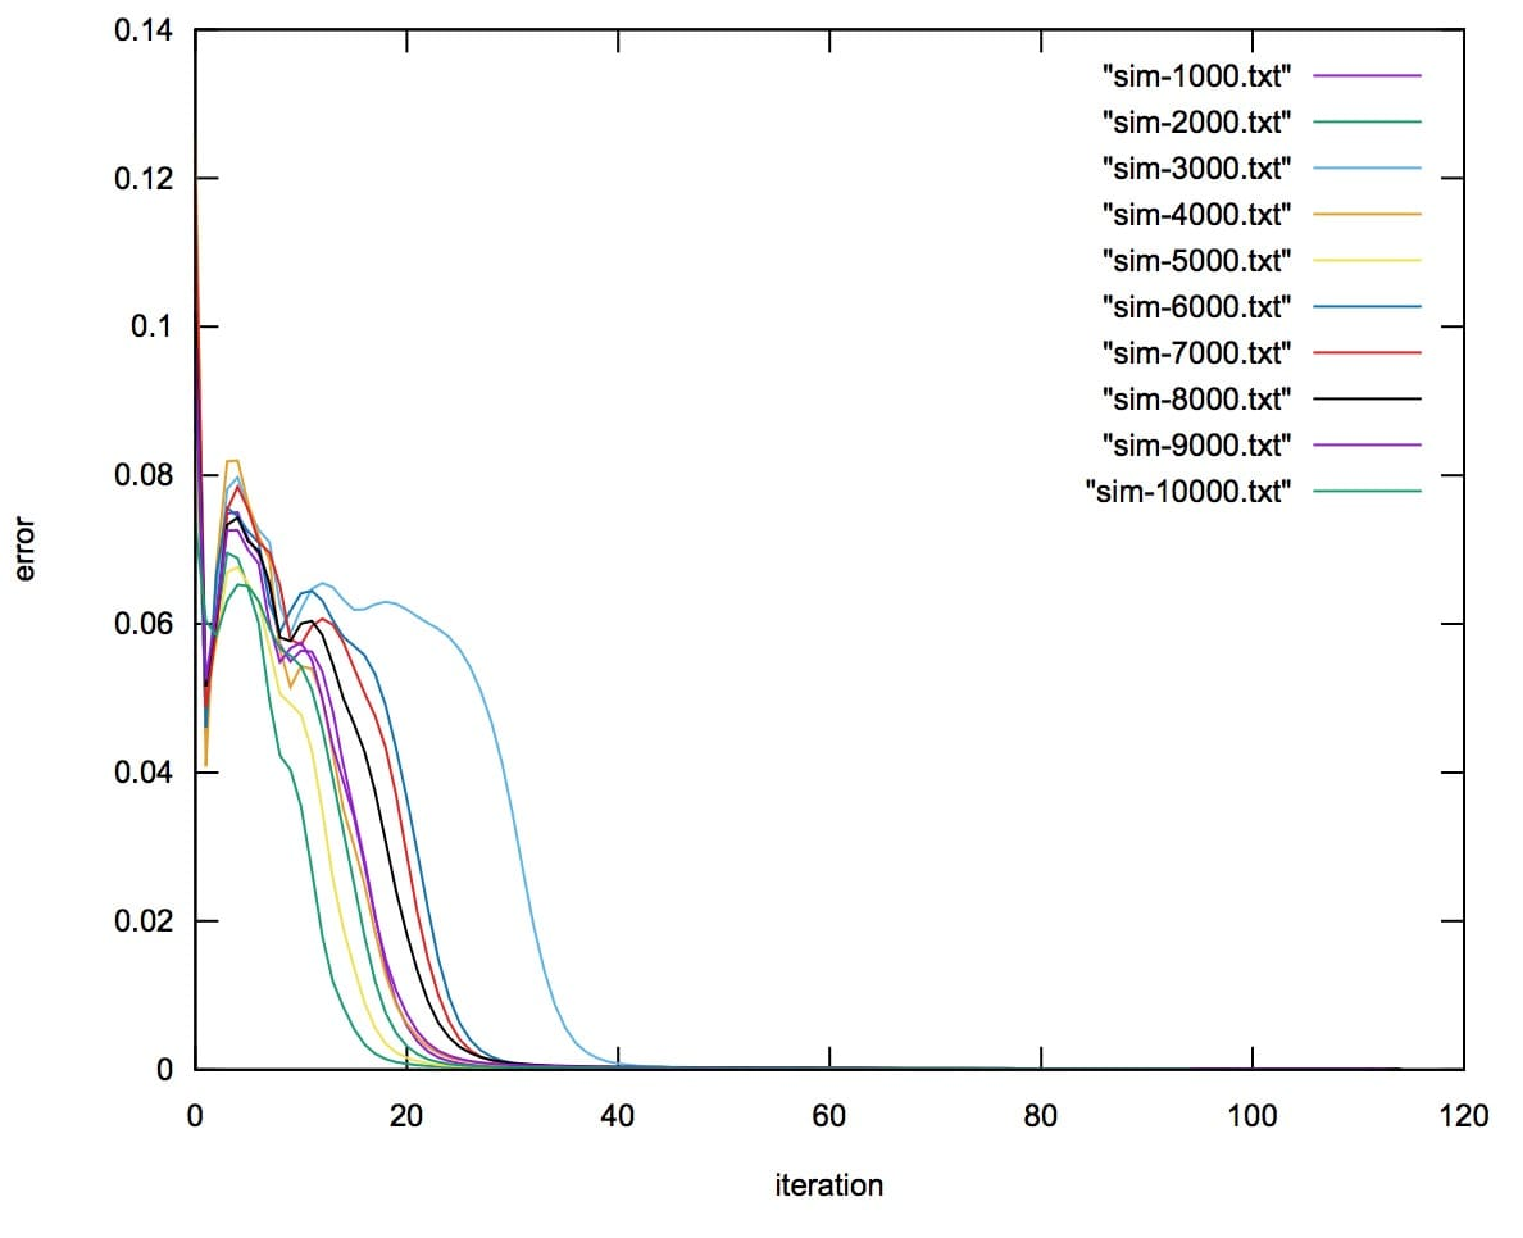
\includegraphics[width=10.0cm]{figs/seeds.pdf}
  \caption{重みを更新する様子}
  \label{fig:level1-1}
 \end{center}
\end{figure}

\begin{figure}[h]
 \begin{center}
  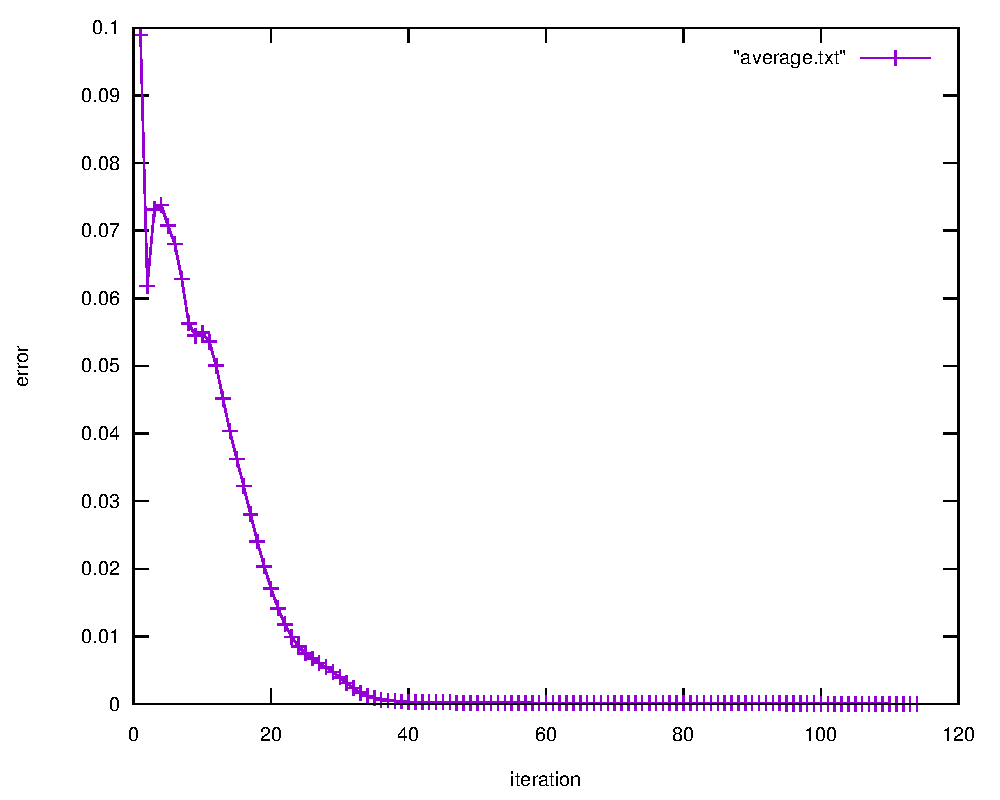
\includegraphics[width=10.0cm]{figs/average.pdf}
  \caption{重みを更新する様子(平均値)}
  \label{fig:level1-2}
 \end{center}
\end{figure}


\subsubsection{考察}
実行結果よりシード値(重み)に関わらず,100回前後の学習でほぼ誤差が0に限りなく近くなることがわかった.

\subsection{「OR問題」を学習させた際の学習の推移(iteration vs error)をグラフ化し、そのグラフ化手順と共に示せ。}

以下のシェルスクリプトも用いて,実験を行った.グラフ作成にはgnuplotを使用した.
\lstinputlisting{./seed.sh}
\lstinputlisting{./sum.sh}
\lstinputlisting{./average.sh}






